\documentclass[final,11pt,oneside,UTF8]{article}
\usepackage{ctex}
\usepackage{float}
\usepackage{geometry}
\usepackage{graphicx}
\usepackage{amssymb}
\geometry{left=1.0cm,right=1.0cm,top=2.5cm,bottom=2.5cm}
\title{Analysis}
\author{AndyShen2006}
\date{Oct.18th.2020}
\begin{document}
\maketitle
\subsection{本解析只包含解析部分以及解析图,不含原题!!!}
\subsubsection{走进重高第一章高分夺冠第五题}
\paragraph{略}
\subsubsection{走进重高第二章高分夺冠第四题}
%    \begin{figure}[ht]
%        \centering
%        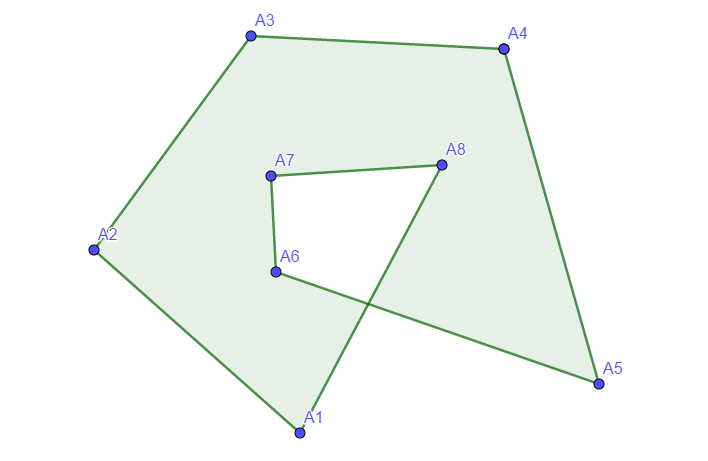
\includegraphics[scale=0.4]{T2B1.jpg}
%    \end{figure}
\paragraph{
这题看着有点绕,但是呢,做法就写在题目里面,所以不难。
考虑用多边形内角和定理,属于比较暴力的做法。
}
\paragraph{
    连结$A_1,A_5$,如图
    \begin{figure}[ht]
        \centering
        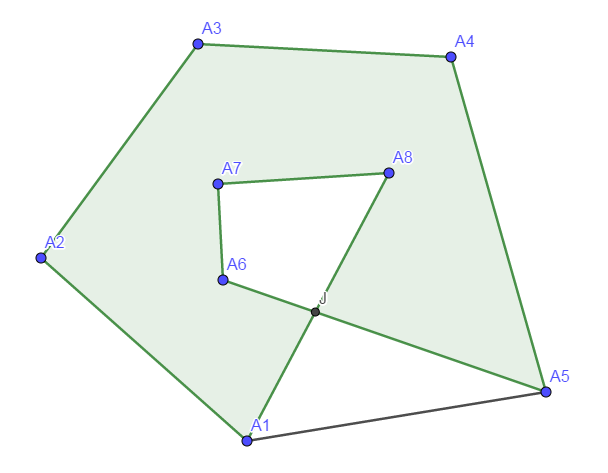
\includegraphics[scale=0.35]{T2A1.png}
    \end{figure}
}
\paragraph{
    由多边形内角和定理易得
    $$\angle JA_1 A_5 +\angle A_1 +\angle A_2 +\cdots +\angle A_5 +\angle JA_5 A_1 = 540^\circ$$
    $$\angle A_6 +\angle A_7 +\angle A_8 +\angle A_6 JA_8 =360^\circ$$
    两式相加,易得
    $$\angle A_1 +\angle A_2 +\cdots +\angle A_8 +\angle JA_1 A_5 +\angle JA_5 A_1 +\angle A_6 JA_8 =900^\circ$$
    $$\angle JA_1 A_5 +\angle JA_5 A_1 +\angle A_6 JA_8 =\angle JA_1 A_5 +\angle JA_5 A_1 +\angle A_1 JA_5 =180^\circ$$
    两式相减,易得
    $$\angle A_1 +\angle A_2 +\cdots +\angle A_8 =720^\circ$$
}
\paragraph{
    之后题目同理,此处不述。
}
\subsubsection{走进重高第三章走进重高第六题}
\paragraph{
    此题过于简单,不述。
}
\subsubsection{走进重高第三章高分夺冠第四题}
\paragraph{
    此类题目都有一个显著特征,都是分割或延长,然后证全等。证完后找等腰三角形
    对于大部分求线段关系题目都是这么去思考的。
}
\paragraph{
    第一小题证法就是题目给的证法,此处不述,只讲第二小题
}
\paragraph{
    第二小题肯定AB+AC=CD,大概猜猜就知道,接着就看为什么吧
    在AF上取一点E,使得AE=AC,然后连接DE\\
    \centering
    $\because AD$平分$\angle FAC$
    $$\therefore \angle EAC=\angle CAD$$
    又$AD=AD,AE=AC$\\
    $$\therefore \triangle ACD \cong \triangle AED(SAS)$$
    $$\therefore \angle AED=\angle ACD=180^\circ -\angle ACB=180^\circ -2\angle B$$
    $$\angle FED=180^\circ -\angle AED=2\angle B$$
    $$\angle EDB=\angle FED-\angle B=\angle B$$
    $$\therefore EB=ED$$
    $$\therefore CD=ED=EB=AE+AB=AB+AC$$
}
\subsubsection{走进重高第三章高分夺冠第五题}
\paragraph{
    第一题没什么好说的,接下来两题全部都要用旋转法解决
}
%\begin{figure}[ht]
%    \centering
%    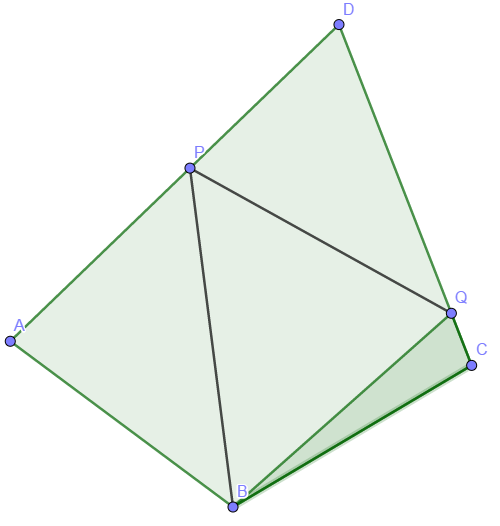
\includegraphics[scale=0.4]{T5B1.png}
%\end{figure}
\paragraph{
    第二题我们看一下$\angle PBQ$和$\angle ABC$的关系,发现前者正好是后者的$\frac{1}{2}$,那么我们
    就是要让$\angle PBQ$所对应三角形和另外一个三角形全等,故我们逆时针旋转$\triangle QBC$,使
    BC与AB重合。
    \begin{figure}[ht]
        \centering
        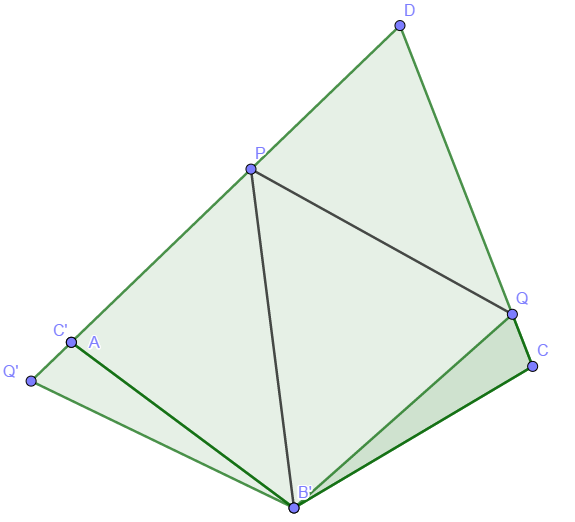
\includegraphics[scale=0.35]{T5A1.png}
    \end{figure}
}
\paragraph{
    $$\because PQ=AP+CQ=AP+C'Q'=PQ',PB=PB,BQ'=BQ$$
    $$\therefore \triangle PBQ\cong \triangle PBQ'(SSS)$$
    $$\angle PBQ=\frac{1}{2}\angle CBQ'=\frac{1}{2}\angle ABC=\frac{1}{2}(180^\circ -\angle ADC)=90^\circ -\frac{1}{2}\angle ADC$$
}
\paragraph{
    第三题的解决方法大致和第二题一样,但是又有点细小的差别,首先因为$\angle ABC$和$\angle ADC$互补
    故$\angle BAD$和$\angle BCD$互补,$\angle BAD=\angle BCQ$,所以我们逆时针$\triangle BQC$使得
    CQ与AD重合是可行的。接着问题就和上题差不多了
    \begin{figure}[ht]
        \centering
        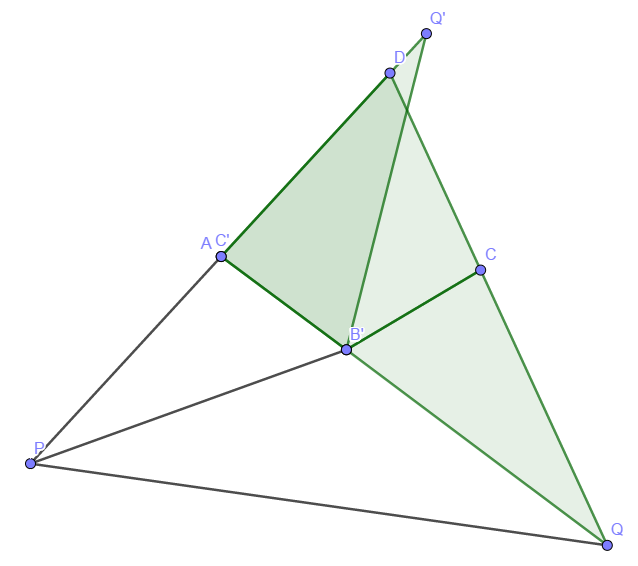
\includegraphics[scale=0.35]{T5A2.png}
    \end{figure}
}
\paragraph{
    $$\because PQ=AP+CQ=AP+C'Q'=PQ',PB=PB,BQ=BQ'$$
    $$\therefore \triangle PBQ\cong \triangle PBQ'(SSS)$$
    $$\angle BPQ=\frac{1}{2}\angle DPQ,\angle Q'=\angle DQA=\angle AQP,\angle AQP=\frac{1}{2}\angle DQP$$
    $$\angle PBQ=180^\circ -(\angle BPQ+\angle BQP)=180^\circ -\frac{1}{2}(\angle DPQ+\angle DQP)=180^\circ - \frac{1}{2}(180^\circ -\angle ADC)=90^\circ+\frac{1}{2}\angle ADC$$
}
\subsubsection{走进重高第六章走进重高第六题}
%\begin{figure}[ht]
%    \centering
%    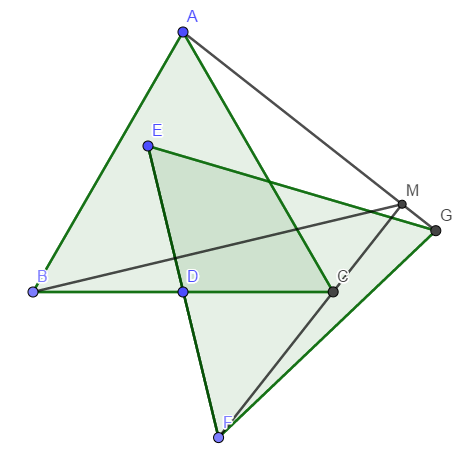
\includegraphics[scale=0.45]{T10B1.png}
%\end{figure}
\paragraph{
    这题首先猜,然后再证,我直觉就感觉这个角是个直角,接着我们就要证这个角是直角
}
\paragraph{
    此类题目首先要看第一小题的问题,第二小题大概率要用到第一小题的结论。如图所示,我们从第一小题
    的经验可以明白,我们应连结AD、CD,由于等边三角形三线合一,我们可以得到垂直。BM没啥用,就不管
}
\begin{figure}[ht]
        \centering
        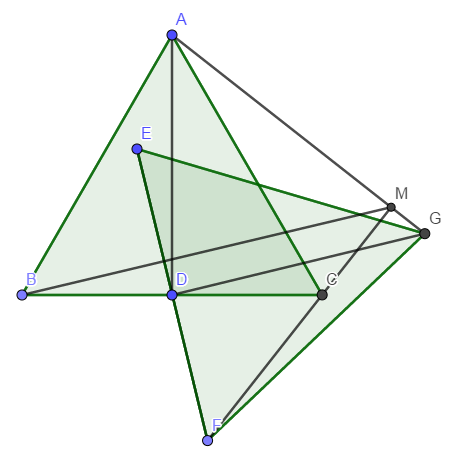
\includegraphics[scale=0.45]{T10A1.png}
\end{figure}
\paragraph{
    观察一下发现$\angle ADM$是个直角,$\angle AMF$是他的对角,如果$\angle AMF$是个直角,那么
    根据四边形内角和定理(四边形内角和$360^\circ$,我们可以得到$\angle DAM$和$\angle DCM$互补
    (其实就是四点共圆),接着我们继续转换,如果$\angle DAM$与$\angle DCM$互补,则$\angle DAM$和
    $\angle DCF$相等,我们这时用到第一小题的结论,因为DC=DF,所以$\triangle DCF$是等腰三角形,
    因为AD=DG,所以$\triangle ADG$是等腰三角形,而$\angle DAM$和$\angle DCF$是这两个三角形的底角
    所以我们只要证明它们的顶角相等即可,而它们的顶角是$\angle ADG$和$\angle FDC$,这两个角同时加上
    $\angle CDG$后都是直角,所以这两个角相等,问题得证。
}
\subsubsection{走进重高第六章高分夺冠第六题}
%\begin{figure}[ht]
%    \centering
%    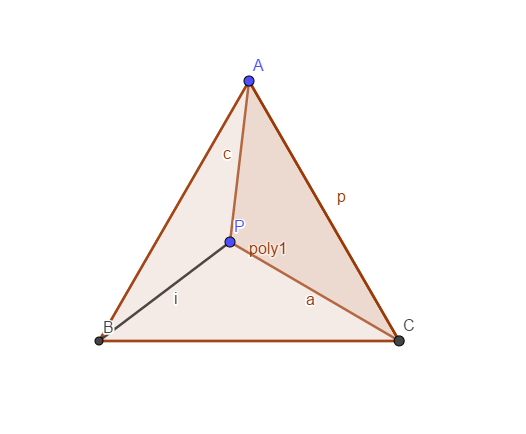
\includegraphics[scale=0.5]{T11B1.jpg}
%\end{figure}
\paragraph{
    这道题目我们先分析,常规办法都不怎么好用,推平行
恐怕也不行,那么就要用到旋转法。
我们将$\triangle ACP$绕顺时针旋转60度,使得AC'
与AB重合,然后连接PP',如图所示
\begin{figure}[ht]
    \centering
    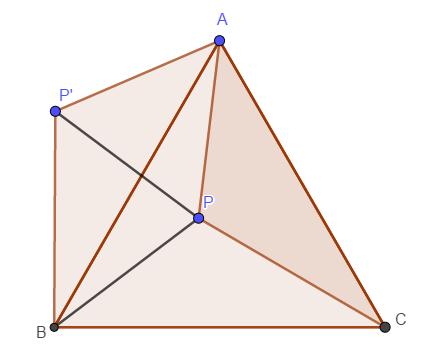
\includegraphics[scale=0.5]{T11A1.jpg}
\end{figure}
}
\paragraph{
    然后由于是旋转,故AP'=AP,已经有两条边相
等了,我们只要再证明除PP'=AP就能够知道
$\triangle BPP'$就是我要的三角形了。
}
\paragraph{为了求得PP'=AP,我要做的是求证三角形
APP'是等边三角形。由于旋转了$60^\circ$,故PAP'=
$60^\circ$,又AP'=AP从而易得$\triangle APP'$
是等边三角形,故PP'=AP',故$\triangle CPP'$就是
AP,BP,CP所组成的三角形。\\
    接着就很简单了
}
$$\angle BPP'=\angle APB-\angle APP'=\angle APB-60^\circ=57^\circ$$
$$\angle APC=180^\circ -\angle APB-\angle BPC=108^\circ$$
$$\angle PP'B=\angle AP'B-\angle AP'P=\angle APC-60^\circ=48^\circ$$
$$\angle PBP'=180^\circ-\angle BPP'-\angle PP'B=75^\circ$$
\end{document}